\documentclass{article}
\usepackage{graphicx} % Required for inserting images
\usepackage{fullpage}
\title{Thapa-F24}
\author{Sahil Thapa}
\date{October 2024}

\begin{document}

\maketitle

\section{Introduction: Sahil Thapa}
I am Sahil Thapa, a PhD in Computer Science. My advisor, Dr. Oluwatosin Oluwadare, guides my research, and I also serve as a graduate research assistant in his bioinformatics lab. My research focuses on utilizing deep learning and artificial intelligence to develop bioinformatics tools, with a current emphasis on splice site detection methods.\\

From a young age, I have enjoyed walking and traveling, a passion instilled in me by my maternal uncle. He often took me to rivers and hills, where we would sit and talk, fostering my love for trekking. I have explored many beautiful places in Nepal, including the Annapurna Mountain Range and the Langtang Circuit. My favorite films are "The Legend of 1900" and "The Forrest Gump."

\begin{figure}[h!]
    \centering
    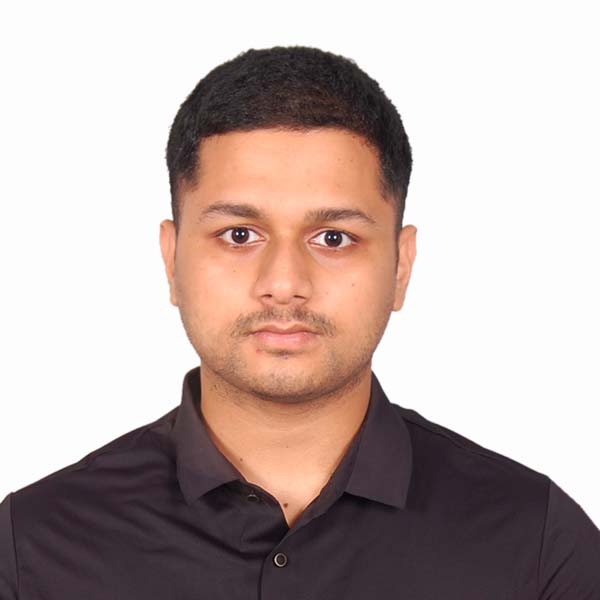
\includegraphics[width=0.5\linewidth]{Sahil_Thapa.jpg}
    \caption{Caption}
    \label{fig:enter-label}
\end{figure}

\section{Output of CNNSplice: Robust models for splice site prediction using convolutional neural networks.}
I explored the following Git repository related to my research: https://github.com/OluwadareLab/CNNSplice.git\\

CNNSplice is a set of deep convolutional neural network models designed for splice site prediction. Developed at the University of Colorado Colorado Springs, CNNSplice aims to efficiently predict true and false splice sites using robust machine learning techniques.

\subsection{test\_logfile\_metrics}
These are Output\_logfile Results of CNNModel.\\
$\{'precision': 0.9027834069851564, 'recall': 0.9206222222222222, 'f1': 0.9111579557303049, 'class_accuracy': 0.9318666666666666, 'accuracy': 0.9318666458129883\}$\\

$\{'precision': 0.9273229649052265, 'recall': 0.9525333333333332, 'f1': 0.9389124679859917, 'class_accuracy': 0.9528, 'accuracy': 0.9527999758720398\}$\\

$\{'precision': 0.9229379328722263, 'recall': 0.9288888888888889, 'f1': 0.925857755161124, 'class_accuracy': 0.944, 'accuracy': 0.9440000057220459\}$\\

$\{'precision': 0.9280761354666826, 'recall': 0.9274666666666667, 'f1': 0.927770831864634, 'class_accuracy': 0.9458666666666666, 'accuracy': 0.9458666443824768\}$\\

$\{'precision': 0.9037206096479873, 'recall': 0.9141333333333334, 'f1': 0.908744230763471, 'class_accuracy': 0.9306666666666666, 'accuracy': 0.9306666851043701\}$

\begin{figure}[h!]
    \centering
    \includegraphics[width=0.5\linewidth]{LogFile.png}
    \caption{LogFile}
    \label{fig:enter-label}
\end{figure}


\section{Questions for me:}


\end{document}
